\subsection{Android}
			\par
				Android es un sistema operativo basado en el núcleo Linux. Fue diseñado principalmente para dispositivos móviles con pantalla táctil, como teléfonos inteligentes, tablets o tabléfonos; y también para relojes inteligentes, televisores y automóviles. Inicialmente fue desarrollado por Android Inc la cual fue fundado en 2003 por Andy Rubin, Rich Miner, Nick Sears y Chris White con el objetivo de desarrollar "dispositivos móviles que están al corriente de la ubicación y preferencias del usuario". En un principio la intención era desarrollar un sistema operativo avanzado para cámaras digitales, pero más tarde se cambió el foco al determinar que el mercado de las cámaras digitales no era lo suficientemente grande. Se redirigirían los esfuerzos a crear un sistema que pudiera competir con Symbian y Windows Mobile.
				
				\begin{figure}[h]
					\centering
					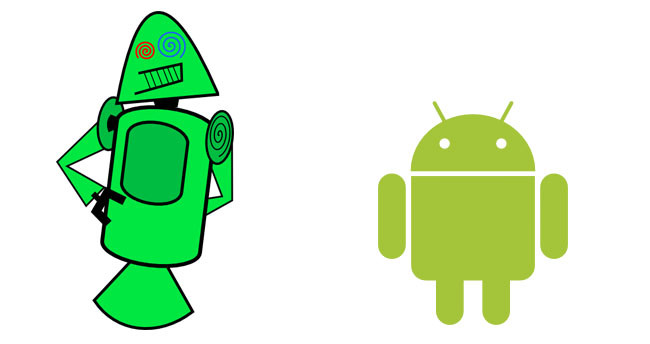
\includegraphics[width=0.65\textwidth]{figure3_androidlogo.jpg}
					\caption{Un diseño preliminar para el logo de Android (izquierda) y el logo final (derecha)}
				\end{figure}
			
			\par \noindent
				 Posteriormente Google respaldó económicamente a Androind Inc. y más tarde, en 2005, la compró. Android fue presentado en 2007 junto la fundación del Open Handset Alliance (un consorcio de compañías de hardware, software y telecomunicaciones entre las que están Texas Instruments, Broadcom Corporation, Nvidia, Qualcomm, Samsung Electronics, Sprint Nextel, Intel, LG, Marvell Technology Group, Motorola, T-Mobile, etc) para avanzar en los estándares abiertos de los dispositivos móviles. El primer móvil con el sistema operativo Android fue el HTC Dream y se vendió en octubre de 2008. Los dispositivos de Android, hoy en día, venden más que las ventas combinadas de Windows Phone e iOS.
			
			\par \noindent
				La versión básica de Android es conocida como Android Open Source Project (AOSP).
			
			\begin{figure}[h]
				\centering
				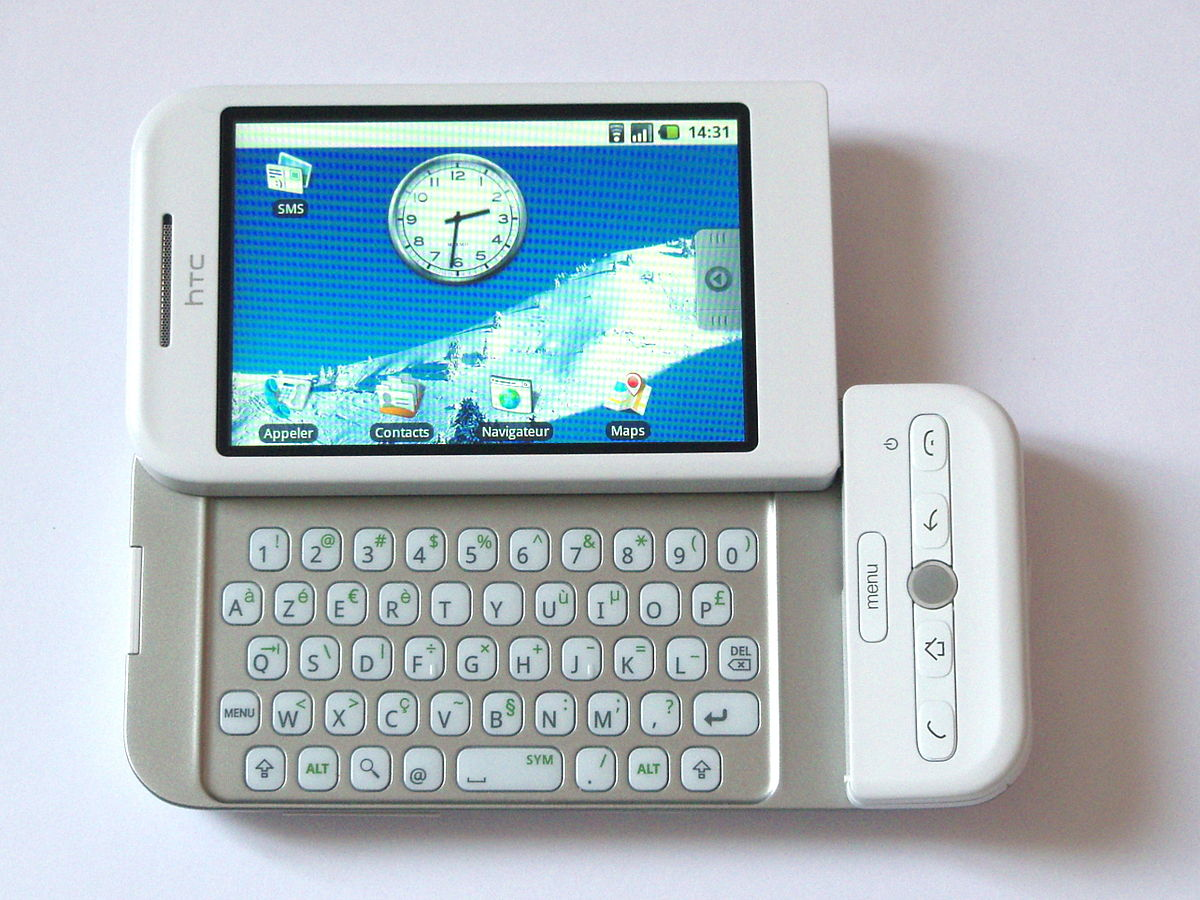
\includegraphics[width=8cm, height=6cm]{figura2_htcdream.jpeg}
				\caption{HTC Dream el primer teléfono con Android}
			\end{figure}
		
		\newpage
		\thispagestyle{plain}
		
		\subsubsection{Android 5.0 Lollipop}
			\par 
				Android Lollipop es una versión del sistema operativo para dispositivos móviles Android. Fue dada a conocer el 25 de junio de 2014 durante el Google I/O 2014 como Android L, Google I/O es una conferencia anual presentada por Google en sus oficinas en Mountain View, California.
				Los cambios más prominentes en Lollipop incluyen una interfaz de usuario rediseñada construida sobre un diseño de lenguaje responsivo denominado como "Material design", así como mejoras en el sistema de notificaciones que permiten que este sea accedido desde la pantalla de bloqueo, y mostrado junto con otras aplicaciones como banners en la parte superior de la pantalla. También se realizaron cambios internos para mejorar y optimizar el rendimiento de consumo de bateria en smartphones.
				
			\begin{figure}[h]
				\centering
				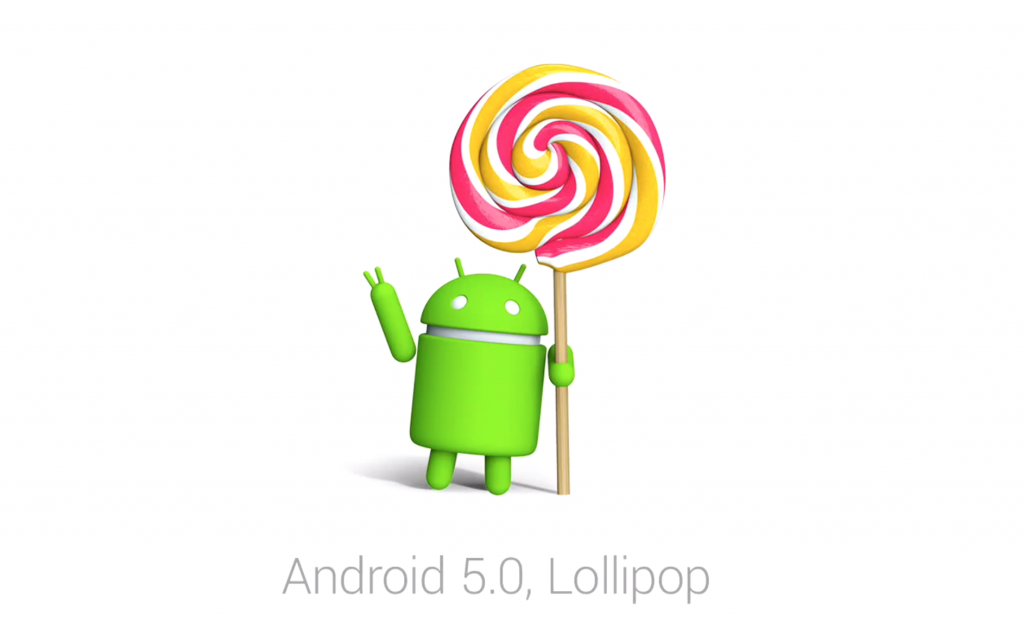
\includegraphics[width=0.5\textwidth]{figura4_lollipop.png}
				\caption{Logo oficial de Android 5.0}
			\end{figure}